\section{字符串}
\begin{frame}[fragile]
  \frametitle{字符串}
  计算机非数值处理的对象经常是字符串数据。如文本检索、文本聚类、文本理解等。

  \begin{itemize}
  \item 串的定义及表示
  \item 串的模式匹配
  \end{itemize}
\end{frame}

\begin{frame}[fragile]
  \frametitle{串 (String)的定义}

  \begin{itemize}
  \item 串是由零个或多个任意字符组成的字符序列。它也是一种特殊的线性表,其数据元
    素仅由一个字符组成,而且它通常是作为一个整体来处理。

例:s="Renmin University",s是串名, Renmin University为串值,其中一个个的字符称
为串的元素。

  \item 请思考如何实现上述串的存储?
  \end{itemize}
\end{frame}

\begin{frame}[fragile]
  \frametitle{字符串的存储}
  \begin{itemize}
  \item 顺序存储: 用一组地址连续的存储单元存储串值中的字符序列。
  \item 链式存储: 考虑到存储密度,可以按块分配。
  \item 在C++/Java等语言中,String就是字符串。在C语言中没有string类型变量,字符串用字符数组表示。
  \end{itemize}
\end{frame}

\begin{frame}[fragile]
  \frametitle{串的模式匹配}
  \begin{itemize}
  \item 设s和t是给定的两个串,在主串s中寻找等于子串t的部分的过程称为模式匹配, t也称为模式。
  \item 如果在s中找到等于t的子串,则称匹配成功,返回t在s中的首次出现的存储位置,否则匹配失败。
  \item 例:

    s="ababcabcacbab"

    t="abcac"
  \end{itemize}
\end{frame}

\begin{frame}[fragile]
  \frametitle{简单的模式匹配}
  \begin{columns}
    \begin{column}[T]{0.5\linewidth}
      s="ababcabcacbab" \\ t="abcac"

      \begin{itemize}
      \item Brute-Force算法
      \end{itemize}
    \end{column}
    \begin{column}[T]{0.5\linewidth}
      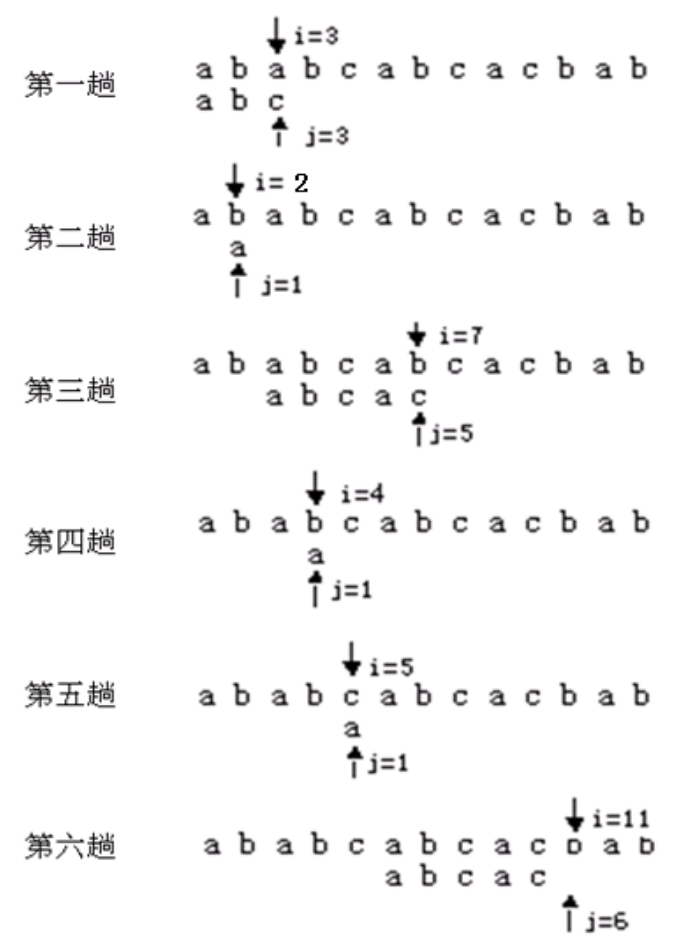
\includegraphics[width=0.9\textwidth]{figs/string/pattern-match.png}
    \end{column}
  \end{columns}
\end{frame}

\begin{frame}[fragile]
  \frametitle{BF算法时间复杂度分析}
  \begin{itemize}
  \item 设串s长度为n,串t长度为m。匹配成功的情况下,考虑两种极端情况。
    \begin{itemize}
    \item 在最好情况下,即每趟不成功的匹配都发生在第一对字符比较时。
    \item 例如:s=“aaaaaaaaaabc”,t=“bc”,设匹配成功发生在$s_i$处。
    \item 在前面i-1趟不成功的匹配中共比较了i-1次,第i趟成功的匹配共比较了m次,所
      以总共比较了i-1+m次。
    \item 所有匹配成功的可能共有n-m+1种,设从si开始与t串匹配成功的概率为$p_i$,
      在等概率情况下$p_i=1/(n-m+1)$,因此最好情况下平均比较的次数是:
      \[\sum_{i=1}^{n-m+1} p_i \times (i-1+m) = \sum_{i=1}^{n-m+1} \dfrac{1}{n-m+1} \times (i-1+m) = \dfrac{(n+m)}{2}\]

    \item 即最好情况下的时间复杂度是$O(n+m)$
    \end{itemize}
  \end{itemize}
\end{frame}

\begin{frame}[fragile]
  \begin{itemize}
  \item 在最坏情况下,即每趟不成功的匹配都发生在t的最后一个字符。
  \item 例如:s=“aaaaaaaaaaab”,t=“aaab”,设匹配成功发生在$s_i$处.
  \item 在前面$i-1$趟匹配中共比较了$(i-1) \times m$次,第$i$趟成功的匹配共比较了
    $m$次,所以总共比较了$i \times m$次,因此最坏的情况下平均比较的次数是:
    \[\sum_{i=1}^{n-m+1} p_i \times (i \times m) = \sum_{i=1}^{n-m+1} \dfrac{1}{n-m+1} \times (i \times m) = \dfrac{m \times (n-m+2)}{2}\]
  \item 即最坏情况下的时间复杂度是$O(n×m)$
  \end{itemize}

  \begin{tcolorbox}[title=为什么BF算法时间性能低?]
    在每趟匹配不成功时存在大量回溯 (每次移动一位开始新的比较)
  \end{tcolorbox}
\end{frame}

\begin{frame}[fragile]
  \frametitle{改进算法}

  \begin{tikzpicture}[box/.style={draw, minimum width=1cm, minimum height=0.8cm}]
    \draw node[minimum width=2cm] (a0) {主串};
    \foreach \i in {1,...,7} {
      \pgfmathtruncatemacro{\x}{\i - 1};
      \draw node[box, right=0 of a\x] (a\i) {A} ;
    }

		\draw node[box, right=0 of a7] (a8) {B}  node[box, right=0 of a8] (a9) {A}  node[box, right=0 of a9] (a10) {A} ;

		\draw node[below=of a0] (b0) {子串}
		node[box, below=of a1] (b1) {A}
		node[box, below=of a2] (b2) {A}
		node[box, below=of a3] (b3) {A}
		node[box, below=of a4, fill=red!50] (b4) {B} ;

	  \draw[draw=red, very thick, <-] (a4) -- ++(0,1);
	  \draw[draw=red, very thick, <-] (b4) -- ++(0,-1);

    \path (a4) edge[draw=red, in=90, out=115, ->, dotted, thick]  (a2);
    \path (b4) edge[draw=red, in=-90, out=-115, ->, dotted, thick]  (b1);
  \end{tikzpicture}

  \begin{itemize}
  \item 改进算法的目的是在每一趟匹配过程中出现不匹配时,向右“滑动”尽可能远的一段
    距离后,继续进行比较。那么,应当滑动多远呢?这正是各个算法各显神通之处!

  \item KMP算法: 由D. E. Knuth,J. H. Morris和V. R. Pratt同时发现

    % \item Boyer-Moore算法
  \end{itemize}
\end{frame}

\begin{frame}[fragile]
  \frametitle{KMP算法}
  利用已经得到的“部分匹配”的结果将模式向右滑动


  视频讲解:\url{https://www.bilibili.com/video/BV1AY4y157yL/}

\end{frame}
